%=========================================================================
% (c) Michal Bidlo, Bohuslav Křena, 2008

\chapter{Úvod}
Počítačové sítě, zejména Internet, v dnešním světě zaujímají jednu z nejvýznamnějších rolí. Počínaje výzkumem a vědeckými experimenty, konče běžným životem většiny lidí. Jen za posledních deset let se počet uživatelů Internetu více než ztrojnásobil z cca jedné miliardy lidí na tři miliardy. Počítačové sítě propujují celý svět a jsou neustále rozšiřovány, vylepšovány a modernizovány. To vede k větším nárokům na použité technologie a zdroje. 

Avšak se zvyšujícím počtem uživatelů roste i počet útoků na různé počítačové sítě, kterými se útočníci snaží získat informace či poškodit oběť. Síťový útok\cite{rfcAttack} je definován jako záměrný akt, kde se entita snaží překonat bezpečnostní služby a porušit bezpečnost systému. Vznikají tím pádem systémy na detekci takovýchto útoků, aby správcí sítí dokázali reagovat na vzniklou situaci.

Jeden z těchto systémů vznikl ve sdružení CESNET s názvem Nemea. Tento framework analyzuje síťový provoz a zaznamenává podezřelé toky jako agregované události do databáze. Na větší síti (stovky až tisíce připojených zařízení) je takovýchto událostí vytvořeno až několik tisíc denně. S tím nastává problém jak dané události jednoduše analyzovat a rozpoznat na jaké události se zaměřit a na které nebrát zřetel.

Cílem této bakalářské práce je vytvořit aplikaci pro vizuální analýzu bezpečnostních událostí na síti monitorované s pomocí frameworku Nemea, tak aby správce sítě dokázal rychle a jednoduše rozpoznat významný útok na síť. Důležitým aspektem vytvořené aplikace je důraz na použití moderních knihoven podporující tvorbu dynamických webových aplikací, které jsou dostupné na různých typech zařízeních. Společně s tím je kladen důraz na uživatelskou přívětivost a jednoduchost prostředí, ve kterém bude probíhat vizuální analýza událostí.

Aplikace bude pracovat s konkrétním formátem dat nazvaný IDEA. Tento formát dat je specifikován sdružením CESNET a slouží jako prostředek pro sdílení dat bezpečnostních událostí mezi různými systémy. Díky tomu lze systém kdykoliv přenést na jiný zdroj databáze než je systém Nemea, např. v rámci sdružení CESNET na systém Warden.

Celou aplikaci navíc bude možno libovolně přizpůsobit tak, aby vyhovovala potřebám daného správce sítě. V aplikaci bude zavedena i technika zvaná {\it drill-down}, která napomáhá rychlé a přehledné analýze velkého množství dat bez ztráty informací o analyzované události.

Aplikace bude integrována do současného Nemea frameworku pod názvem Nemea Dashboard a bude s ním společně distribuována jako front~end celého systému.

\chapter{Monitoring síťě}

V majoritních sítích jako např. páteřní či firemní sítě je téměř nutností monitorovat provoz na síti, abychom byli informování o jejím aktuálním stavu.

Monitoring lze rozdělit do dvou částí. Aktivní a pasivní způsob.

\section{Nemea}

Network Measurements Analysis, zkráceně Nemea, je framework, který dovoluje seskládat systém pro automatizovanou analýzu toků získaných ze síťového monitoringu v reálném čase. Systém se skládá z oddělených stavebních bloků nazývané moduly. Tyto jednotlivé moduly jsou následně propojeny pomocí rozhraní.

Moduly jsou nezávislé pracovní jednotky, které obecně přijímají proud dat na svých vstupech, zpracují či zanalyzují daná data a následně je odešlou ze svých výstupních rozhraní jako proud dat pro další moduly. Modul může například tvořit statistiky o přijatých datech a na základě těchto statistik detekovat určité typy síťového útoku. Detekovaný útok je popsán datovým záznamem, který je odeslán přes výstupní rozhraní dalším modulům, které s daným záznamem dále pracují, např. jej uloží v IDEA formátu (viz sekce \ref{sec:idea}) do databáze nebo ze získaných statistik dokáží detekovat anomálie v síťovém provozu a dokáží tak jednotlivé pokusy od jednoho útočníka agregovat a zpracovat jej jako jediný útok skládající se z několika desítek až stovek pokusů o útok, které odděleně nemají význam a administrátor sítě by je snadno přehlédl nebo ignoroval.

Jednotlivé moduly nemají osamoceně velký význam, ale pokud tyto moduly spojíme ve složitější systém, získáme komplexní nástroj na aktivní analýzu síťových dat schopný detekovat a identifikovat útoky na monitorovanou síť, který následně detekované útoky uloží do databáze a webová aplikace, kterou v této práci navrhujeme, uložené útoky zobrazí.

Nemea je také schopná přístupu ``store-and-ex-post'', který lze vidět na obrázku \ref{fig:nemea-schema}. Jsou zde dva moduly spojené jedním rozhraním. První modul čte záznamy toků ze souboru a druhý modul počítá statistiky těchto přečtených toků. 
\begin{figure}[ht]
  \centering
    
\includegraphics[width=0.5\textwidth]{fig/nemea-basic.pdf}
  \caption{Minimální příklad Nemea systému} \label{fig:nemea-schema}
  
\end{figure}

Z takto základních bloků lze postavit i velmi komplexní systém jak je vidět na obrázku \ref{fig:nemea-example-2}, kde jsou data přijímána v reálném čase z IPFIX\cite{ipfix} kolektoru

\begin{figure}
  \centering
    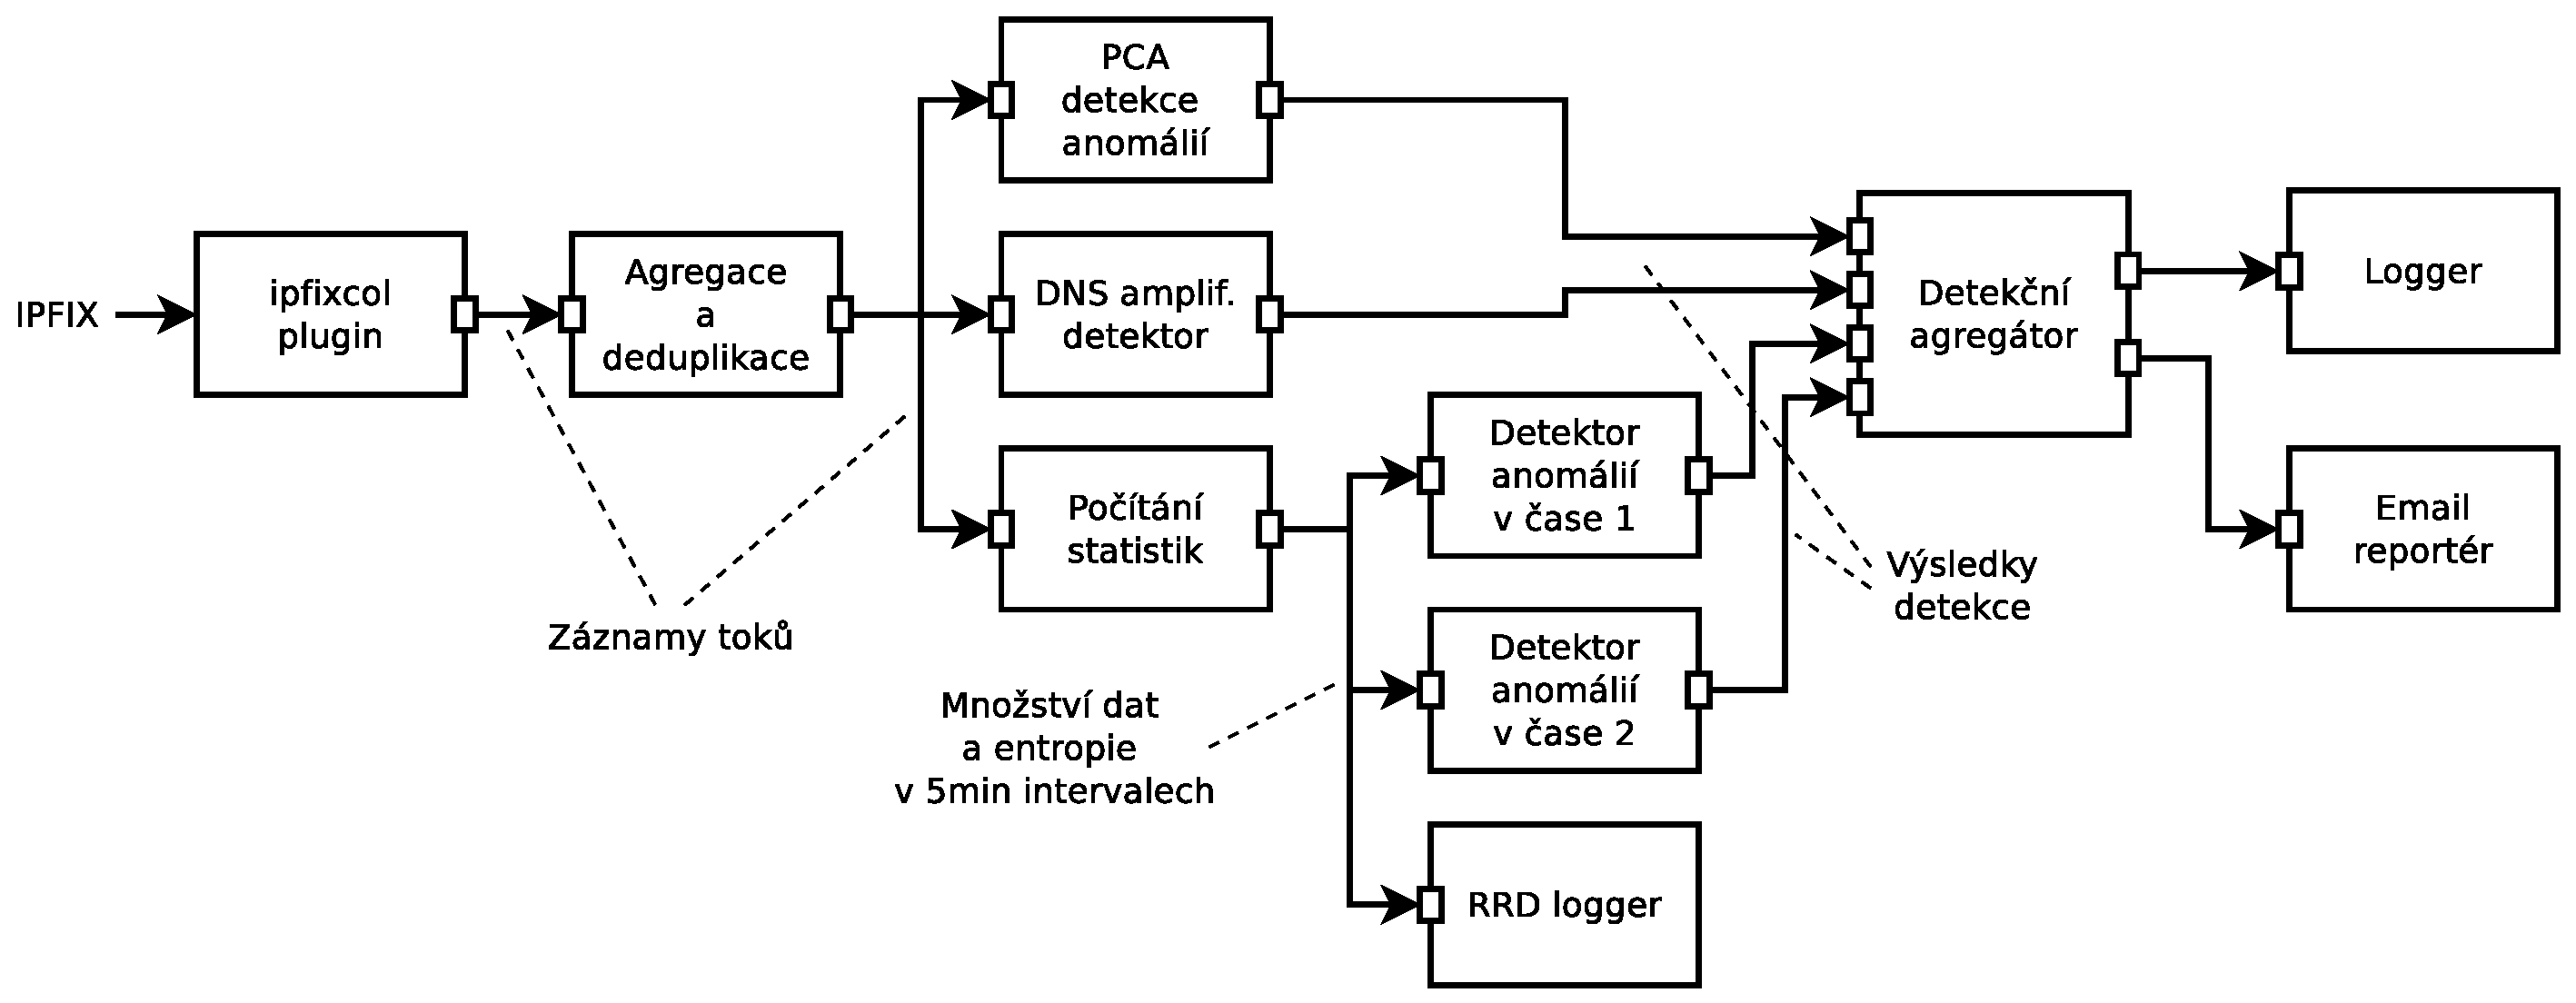
\includegraphics[width=1\textwidth]{fig/nemea-example-2-cz.eps}
  \caption{Minimální příklad Nemea systému} \label{fig:nemea-example-2}
  
\end{figure}




\subsection{Hlavní komponenty}

\subsubsection{Modul}

\subsubsection{libtrap}

\subsubsection{UniRec}

\section{IDEA}
\label{sec:idea}

\section{Další monitorovací systémy}

\chapter{Technologie}
\section{Dostupné technologie}
\section{Výběr technologií}
\section{Zvolené technologie}

\chapter{Architektura aplikace}
\section{REST API}
\section{Databáze událostí}
\section{GUI}

\chapter{Implementace}
\section{Backend}
\section{Frontend}
\section{Zabezpečení}
\section{Distribuce}

\chapter{Dosažené výsledky}
\section{Názory uživatelů}
\section{Nasazení v praxi}

\chapter{Závěr}
Závěrečná kapitola obsahuje zhodnocení dosažených výsledků se zvlášť vyznačeným vlastním přínosem studenta. Povinně se zde objeví i zhodnocení z pohledu dalšího vývoje projektu, student uvede náměty vycházející ze zkušeností s řešeným projektem a uvede rovněž návaznosti na právě dokončené projekty.

%=========================================================================
